\section{Industrie 4.0}
\label{sec:industrie40}

Industrie 4.0, oft auch synonym als „Die vierte industrielle Revolution“ oder „Smart Industry“ bezeichnet, ist eine Vision und der Name des aktuellen Trends hin zu einer vermehrten Automatisierung und zunehmenden Datenaustauschs in der Fertigungstechnik [\cite{industrie40anderl}]. Der Ursprung von Industrie 4.0 geht auf eine Initiative der Bundesregierung und der deutschen Fertigungsindustrie zurück.

Die wesentlichen Charakteristiken der verschiedenen „Stufen“ von Industrie 1.0 bis Industrie 4.0 sind in Grafik \ref{fig:Industrie1.0-zu-4.0} abgebildet. Dabei wird die Entwicklung von den Grundzügen der Automatisierung und Mechanisierung bis hin zur aktuellen vernetzten, selbst gesteuerten und selbst optimierenden Produktion dargestellt.
%
\begin{figure}[htbp]
	\centering\includegraphics[width=1.0\textwidth]{images/02/Industrie1.0-zu-4.0.png}
    \caption{Weg von Industrie 1.0 zu Industrie 4.0 [\cite{wegIndustrie10zu40}]}
    \label{fig:Industrie1.0-zu-4.0}
\end{figure}

Um weiter auf die konkreten Charakteristiken von Industrie 4.0 einzugehen und wie sie sich von dem vorhergehenden Status quo absetzt, seien hier einige dieser Punkte aufgeführt [\cite{industrie40explained}]:
\begin{itemize}
    \item Überbrückung der physischen und digitalen Welt durch Cyber-Physische Systeme (CPS), ermöglicht durch IIoT (siehe Kapitel \ref{subsec:iot_iiot})
    \item Mehr und weitreichendere Automatisierung als in der dritten industriellen Revolution
    \item Selbstgesteuerte Fabriken (Smart Factories)
    \item Closed-Loop-Regelsysteme und -Datenmodelle bei denen der Output wieder in das System zurückgegeben wird, um die zukünftige Funktion anzupassen
    \item Steuerung von Produktionsschritten durch intelligente Produkte und eine damit einhergehende Verlagerung weg von einem zentralen Steuerungssystem und hin zu einer verteilten und adaptiven Steuerung
    \item Benutzergesteuerte Personalisierung/Anpassung von Produkten und die damit verknüpfte und tiefgreifende Flexibilität in der Fertigung
    \item Wandelbare und anpassungsfähige Fabriken
\end{itemize}

Dabei sei ein besonderer Fokus auf die Relevanz von Industrial IoT (siehe Kapitel \ref{subsec:iot_iiot}) gelegt, welches viele der anderen Punkte überhaupt erst ermöglicht, sowie auf die weitreichende Automatisierung und benutzergesteuerte Anpassung, welche beide eine vorherrschende Rolle in dieser Arbeit haben.\\
Doch natürlich ist IIoT nicht die einzige Grundlage, welche diese neuartigen Möglichkeiten begünstigt. Daneben sind auch Technologien wie Cloud-Computing und -Plattformen (wie Amazon Web Services (AWS), Microsoft Azure und Google Cloud), Big Data (Advanced Data Analytics, Data Lakes, Edge Intelligence) mit künstlicher Intelligenz (KI), Datenanalyse, Datenspeicherung und Rechenleistung an den Endpunkten von Netzwerken (Edge Computing), Mobile Endgeräte, Datenkommunikation und Netzwerktechnologien, Veränderungen unter anderem auf der Ebene von Mensch-Maschine-Schnittstellen (engl.: Human-Machine-Interface, kurz: HMI) und Supervisory Control and Data Acquisition (SCADA), Manufacturing Execution Systems (MES), Enterprise Resource Planning (ERP, wird i-ERP), speicherprogrammierbare Steuerungen (SPS), Sensoren und Aktoren, Microelectromechanical Systems (MEMS) und Transducer (dt.: Wandler, Umsetzer, Umrichter und Konverter) und innovative Datenaustauschmodelle eine wichtige Grundlage, auf der Industrie 4.0 aufgebaut ist [\cite{industrie40explained}]. Neben diesen Grundsteinen gibt es noch zahlreiche Weitere, von denen die für diese Arbeit besonders relevanten in Kapitel \ref{cha:grundlagen} näher beschrieben werden. Die meisten dieser Begriffe sollen hier jedoch nur der Vollständigkeit halber und zur grundlegenden Einordnung erwähnt werden.

Wie diese Technologien in eine Hierarchie einzuordnen sind und wie sie zusammenarbeiten, um zu einer industriellen Transformation zu führen, sei in Grafik \ref{fig:Industrie40transformation} kurz angeschnitten. Wie dort zu sehen ist, decken die für Industrie 4.0 relevanten Neuerungen und Aspekte die gesamte Automationspyramide ab.
%
\begin{figure}[htbp]
	\centering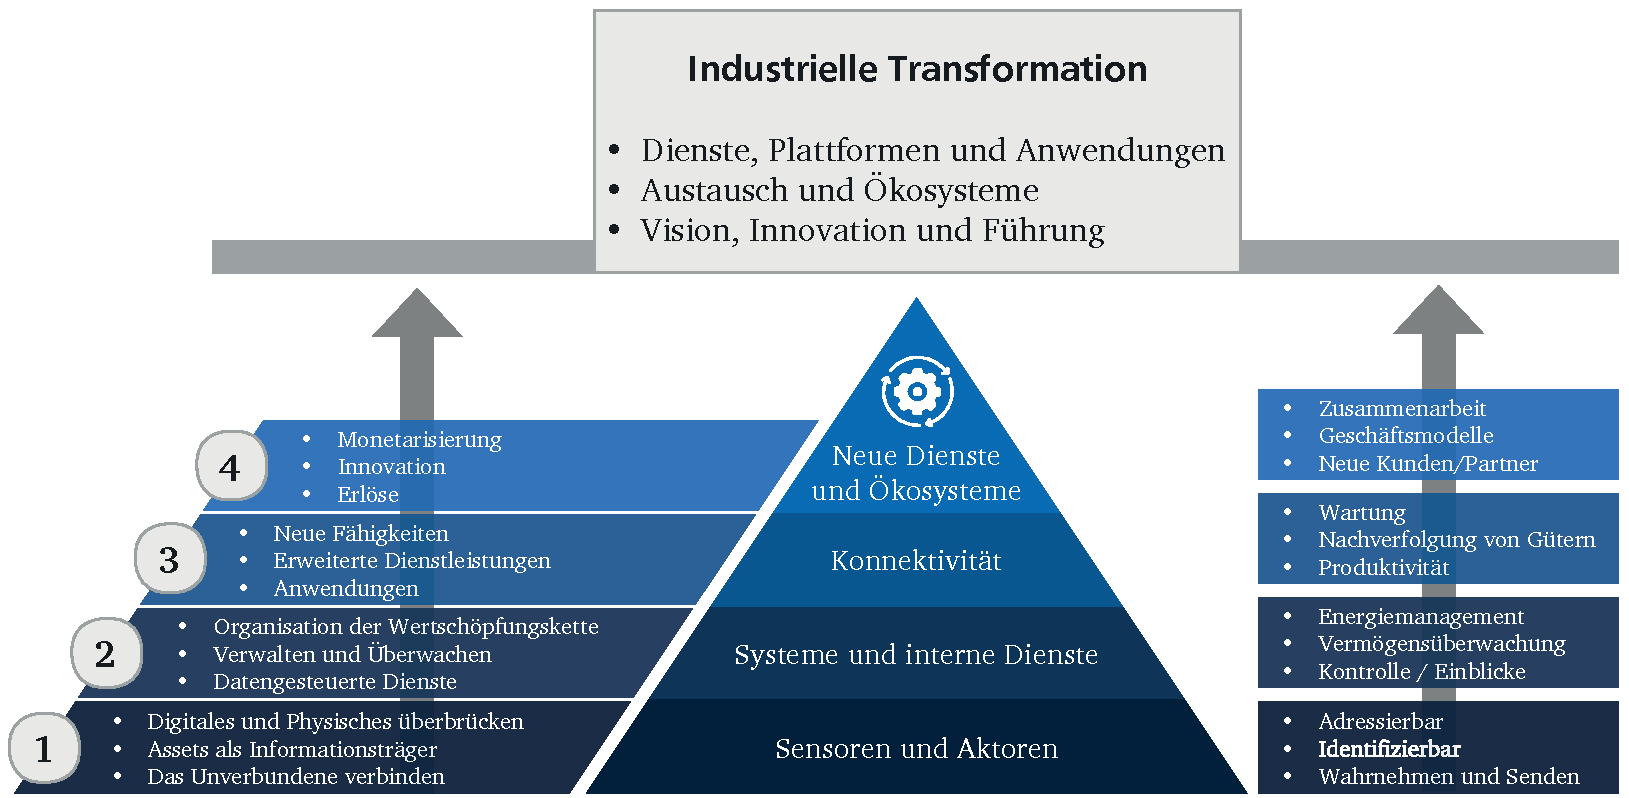
\includegraphics[width=1.0\textwidth]{images/02/Industrie40transformation.pdf}
    \caption{Von der Automatisierungspyramide zur industriellen Transformation mit Industrie 4.0 [eigene Abbildung nach \cite{industrie40explained}]}
    \label{fig:Industrie40transformation}
\end{figure}

\subsection{Kategorisierung von Industrie 4.0}
\label{subsec:industrie40kategorien}

Diese Technologien lassen sich grob in neun Kategorien einteilen, welche alle neuerlich größere Fortschritte erlebt haben. Industrie 4.0 lässt sich daher als Konvergenz dieser neun Teilbereiche von digitalen Industrietechnologien bezeichnen [\cite{industrie40explained}]. Diese Teilbereiche sind im Folgenden ausgeführt:

\WarningsOff[paralist]
\subsubsection*{Big Data und Datenanalyse}
\begin{compactenum}[•]
    \item Unterstützung bei der Entscheidungsfindung in Echtzeit
    \item Maschinenausfälle vorhersagen und Ausfallzeiten reduzieren
    \item Vollständige Auswertung der verfügbaren Daten
    \item Optimierung von Prozessen
\end{compactenum}

\subsubsection*{Cloud}
\begin{compactenum}[•]
    \item Auslagerung von Berechnungen
    \item Verlagerung von Infrastruktur nach Außen
    \item Rasante und flexible Skalierung
    \item Verwaltung großer Datenmengen in offenen Systemen
\end{compactenum}

\subsubsection*{Virtuelle/Erweiterte Realität}
\begin{compactenum}[•]
    \item Geführte Wartung, Support und Logistik
    \item Risikofreie Mitarbeiterschulung
    \item Verbesserung der Kundenerfahrungen
    \item Realitätsnahe Simulation und digitaler Zwilling
\end{compactenum}

\subsubsection*{Horizontale und vertikale Integration}
\begin{compactenum}[•]
    \item Datenaustausch zwischen allen Gebieten bis hin zum Endbenutzer und Kunden
    \item Unternehmensübergreifende Datenintegration auf Basis von Datenübertragungsstandards
    \item Voraussetzung für eine voll automatisierte Wertschöpfungskette
\end{compactenum}

\subsubsection*{Cybersicherheit}
\begin{compactenum}[•]
    \item Größere Netze und horizontale Integration bieten mehr Angriffsfläche
    \item Betrieb in Netzwerken und offenen Systemen
    \item Hohe Vernetzung zwischen Maschinen, Systemen und Produkten
\end{compactenum}

\subsubsection*{Simulation}
\begin{compactenum}[•]
    \item Simulation von Wertschöpfungsnetzwerken
    \item Optimierung auf Basis von Echtzeitdaten intelligenter Systeme
    \item Reduzierung der Verschwendung von Zeit und Ressourcen und Erhöhung der Effizienz in der Fertigung
\end{compactenum}

\subsubsection*{Industrielles Internet}
\begin{compactenum}[•]
    \item Verbesserte Sicherheit und Fehleranfälligkeit
    \item Multidirektionale Kommunikation zwischen vernetzten Objekten
    \item Verbesserte und intelligente Konnektivität zwischen Geräten, Maschinen und Produkten
\end{compactenum}

\subsubsection*{Additive Fertigung}
\begin{compactenum}[•]
    \item 3D Druck
    \item Schnelle Prototypentwicklung
    \item Einfache und schnelle Herstellung von Einzel- und Ersatzteilen
    \item Dezentrale 3D-Druckanlagen zur Reduzierung von Transportwegen und Lagerbeständen
    \item Konsolidieren einer Baugruppe zu einem einzigen Teil
    \item Reduzierung der Kosten und Erhöhung der Geschwindigkeit kleiner Produktionsserien
\end{compactenum}

\subsubsection*{Fortschrittliche Robotik}
\begin{compactenum}[•]
    \item Autonome Industrieroboter
    \item Kooperierende und kommunizierende Roboter
    \item Zahlreiche integrierte Sensoren
    \item Standardisierte Schnittstellen
\end{compactenum}
\WarningsOn[paralist]

\subsection{Design-Prinzipien von Industrie 4.0}
\label{subsec:industrie40design}

Um nun Software (oder auch Hardware) zu entwickeln, welche in diesen Kontext passt, ist es hilfreich, Prinzipien zu identifizieren, welche aus den Charakteristiken von Industrie 4.0 hervorgehen und welche dann als Richtlinien genutzt werden können [\cite{industrie40design}]. Neben den oben genannten Teilbereichen lässt sich Industrie 4.0 auch in verschiedene Komponenten einteilen. Im Gegensatz zu den Teilbereichen orientieren diese sich eher an den zuvor genannten Charakteristiken von Industrie 4.0. Hinzu kommt hier das Internet of Services (IoS), welches das Prinzip abbildet, dass alles als ein abgekapselter, standardisierter und interoperabler Service verpackt und über das Internet zugänglich gemacht wird.\\
Welche Design-Prinzipien sich von diesen Komponenten ableiten, wird in Tabelle \ref{tab:industrie40komponenten} aufgezeigt und darauffolgend wird auf jede dieser Prinzipien eingegangen.
%
\bgroup
\def\arraystretch{1.5}
\vspace{5mm}\begin{table}[htbp]
    \centering
    \begin{tabularx}{156mm}{@{}p{37mm}|*4{>{\centering\arraybackslash}X}@{}}
        \rowcolor{dikblue} & \mbox{\color{white}\textbf{Cyber-Physi-}} \newline \mbox{\color{white}\textbf{sche Systeme}} & \hspace{1mm} \mbox{\color{white}\textbf{Smart}} \newline \mbox{\color{white}\textbf{Factory}} & \mbox{\color{white}\textbf{Internet of}} \newline \mbox{\color{white}\textbf{Things}} & \mbox{\color{white}\textbf{Internet of}} \newline \mbox{\color{white}\textbf{Services}} \\
        Dezentralisierung   & \FeatureTrue  & \FeatureTrue  & \FeatureFalse & \FeatureFalse \\ \hline
        Virtualisierung     & \FeatureTrue  & \FeatureTrue  & \FeatureFalse & \FeatureFalse \\ \hline
        Interoperabilität   & \FeatureTrue  & \FeatureTrue  & \FeatureTrue  & \FeatureTrue  \\ \hline
        Serviceorientierung & \FeatureFalse & \FeatureFalse & \FeatureFalse & \FeatureTrue  \\ \hline
        Modularität         & \FeatureFalse & \FeatureFalse & \FeatureFalse & \FeatureTrue  \\ \hline
        Echtzeitfähigkeit   & \FeatureFalse & \FeatureTrue  & \FeatureFalse & \FeatureFalse
    \end{tabularx}
    \caption{Design-Prinzipien von Industrie 4.0 Komponenten [\cite{industrie40design}]}
    \label{tab:industrie40komponenten}
\end{table}
\egroup

\subsubsection{Dezentralisierung}

Eine zentralisierte Überwachung und Steuerung wird aufgrund zunehmend diversifizierter Produktangebote erschwert; ebenso über mehrere Fertigungsstandorte hinweg. Eine Dezentralisierung dieser Systeme kann mithilfe von eingebetteten Computern erreicht werden. Diese können dann eigenständig Entscheidungen treffen, sodass nur im Fehlerfall die Verantwortlichkeiten auf eine übergeordnete Ebene übertragen werden müssen [\cite{industrie40dezentral}]. Um auch dezentral eine Verwaltung und Qualitätssicherung sicherzustellen, können beispielsweise Radio-frequency identification (RFID) Chips verwendet werden [\cite{industrie40design}].

\subsubsection{Virtualisierung}

Durch die Kopplung von virtuellen Anlagen- und Simulationsmodellen an die Sensordaten physischer Systeme, kann eine Anlage über Virtualisierung überwacht werden. Es wird also eine virtuelle Nachbildung der realen Welt konstruiert, in welcher der Zustand der physischen Anlagen gespiegelt wird. So kann nicht nur eine bessere Überwachung stattfinden, sondern auf dem digitalen Zwilling können auch Simulationen und Analysen vollzogen werden und der Benutzer wird im Umgang mit der Maschine unterstützt [\cite{digitalerZwilling}].

\subsubsection{Interoperabilität}

Ein zentraler Bestandteil von Industrie 4.0 ist Interoperabilität, denn bei einem hohen Grad an Vernetztheit ist es erforderlich, dass unterschiedliche Geräte von verschiedenen Herstellern alle miteinander kommunizieren können. Da eine einheitliche Kommunikation im Wesentlichen von verwendeten Standards abhängt, wurde von der \textit{Deutschen Kommission Elektrotechnik Elektronik Informationstechnik in DIN und VDE} schon 2013 die „Deutsche Normungsroadmap Industrie 4.0“ [\cite{industrie40norm}] herausgegeben, welche Normen für das Themengebiet Industrie 4.0 definiert. In den vergangenen Jahren wurde dieses Dokument mehrfach überarbeitet und liegt nun in der vierten Version vor.

\subsubsection{Serviceorientierung}

Für die Serviceorientierung werden die einzelnen Funktionen einer Anlage oder Anlagenkomponente zu einzelnen „Services“ abgekapselt. So wird ein hohes Maß an Modularität gewährleistet, da die Nutzer dieser Services sich so besser entscheiden können, welche Funktionen genutzt werden und welche nicht [\cite{industrie40service}]. Aufgrund der isolierten Natur dieser Services ist es außerdem möglich, die Fähigkeiten der Anlange schnell an einen geänderten Bedarf anzupassen.

\subsubsection{Modularität}

Um sich flexibel an die Veränderung von Anforderungen anpassen zu können, ist ein modulares System nötig. Die einzelnen Module können dann verändert, erweitert, oder gänzlich ausgetauscht werden, um die Fähigkeiten des Gesamtsystems anzupassen. Dies ist sowohl wichtig, um sich kurzfristigen Veränderungen wie Kundenwünschen anzupassen, als auch um regelmäßige oder geplante Veränderungen zu erleichtern. Wichtige Bestandteile hierfür sind standardisierte Soft- und Hardwareschnittstellen sowie ein automatisierter Findungs- und Kopplungs-Mechanismus. Im Idealfall sollte damit eine Modularität nach dem Plug\&Play-Prinzip möglich sein [\cite{industrie40modularity}].\\
Die zuvor erwähnten Punkte der Interoperabilität und Serviceorientierung spielen eine zentrale Rolle bei der Umsetzung eines modularen Systems.

\subsubsection{Echtzeitfähigkeit}

Um Daten in Echtzeit zu sammeln und zu analysieren, sowie um kurzzeitig auf Probleme und Ausfälle zu reagieren, muss der Zustand der Maschinen durchgehend überwacht werden. Die Daten werden direkt an entsprechende Programme weitergegeben und verarbeitet.
